\chapter{Implementación}

En este capítulo, nos centraremos en la implementación del diseño detallado en el capítulo anterior. 

Describiremos los pasos y técnicas utilizadas para llevar a cabo la construcción de la plataforma, desde la configuración del entorno de desarrollo hasta la integración de los diferentes componentes del sistema. 

También se detallará el proceso de programación, las herramientas empleadas y las decisiones técnicas tomadas para asegurar que el diseño se traduzca eficazmente en una solución funcional. 

Además, abordaremos los retos encontrados durante la implementación y las soluciones adoptadas.




\newpage

\section{Sistema operativo}

Para el desarrollo de la plataforma se ha utilizado el sistema operativo Ubuntu, en concreto su versión 24.04.

Ubuntu es una distribución de Linux orientada al software libre y a la facilidad de uso. Es gratuita, fácil de instalar y ampliamente utilizada en el ámbito académico, especialmente en titulaciones relacionadas con la informática como la nuestra.

Además, gracias al uso de un script ejecutable, es posible instalar fácilmente todas las dependencias necesarias para el proyecto, lo que facilita la configuración del entorno de desarrollo en otros equipos.

\begin{figure}[H]
    \centering
    
\includegraphics[width=1\linewidth]{imagenes/ubuntuLogo.jpg}
    \caption[\textbf{Logo de Ubuntu}.]{\textbf{Logo de Ubuntu}. Una de las mejores distribuciones de Linux, gratuita e ideal para programadores. \href{https://www.drouiz.com/wp-content/uploads/2015/12/ubuntu-logo2.jpg}{https://www.drouiz.com/wp-content/uploads/2015/12/ubuntu-logo2.jpg}.}
    \label{logo-ubuntu}
\end{figure}

\newpage


\section{GitHub}

Para mantener nuestro trabajo seguro, con posibilidad de recuperar versiones anteriores y documentar adecuadamente los cambios realizados, utilizamos GitHub como sistema de control de versiones.

GitHub permite crear un repositorio que contiene todos los archivos del proyecto. Este repositorio puede clonarse en cualquier ordenador, facilitando así el trabajo colaborativo o desde distintos entornos. Una de sus principales funcionalidades es la posibilidad de crear distintas ramas, lo que permite, por ejemplo, desarrollar nuevas funcionalidades o corregir bugs de forma aislada. Posteriormente, estos cambios pueden fusionarse con la rama principal, conservando un historial detallado de versiones.

Gracias a GitHub, no solo almacenamos nuestro trabajo de forma remota en la nube, sino que también facilitamos el control de cambios, la colaboración con otras personas y la organización del desarrollo del proyecto.

El enlace al repositorio del proyecto es el siguiente: \url{https://github.com/juuaann03/TFG}


\begin{figure}[H]
     \centering
     
\includegraphics[width=1\linewidth]{imagenes/gitHubLogo.jpg}
     \caption[\textbf{Logo de GitHub}.]{\textbf{Logo de GitHub}. GitHub es una plataforma gratuita de desarrollo colaborativo que permite a los programadores gestionar proyectos y compartir códigos de manera eficiente y segura. \href{https://cdn.prod.website-files.com/5f5a53e153805db840dae2db/64e79ca5aff2fb7295bfddf9_github-que-es.jpg}{https://cdn.prod.website-files.com/5f5a53e153805db840dae2db/64e79ca5aff2fb7295bfddf9\_github-que-es.jpg}.}
     \label{logo-github}
 \end{figure}


\newpage


\section{Entorno de desarrollo}

Para el desarrollo de la plataforma se ha utilizado un entorno de desarrollo integrado (IDE), concretamente Visual Studio Code.

Un entorno de desarrollo proporciona un conjunto de herramientas que facilitan la programación, tales como la visualización estructurada de archivos, resaltado de sintaxis, autocompletado, depuración, y la integración directa con sistemas de control de versiones como Git y GitHub.

Visual Studio Code es un IDE moderno, ligero y altamente configurable, compatible con una amplia variedad de lenguajes de programación. Ofrece una gran cantidad de extensiones, incluyendo soporte avanzado para Python, HTML, JavaScript... Además, su integración con Git y GitHub permite realizar operaciones de control de versiones de forma sencilla y eficiente desde el propio editor.

Su interfaz intuitiva y su flexibilidad lo convierten en una herramienta ideal para el desarrollo de nuestra plataforma.

\begin{figure}[H]
     \centering
    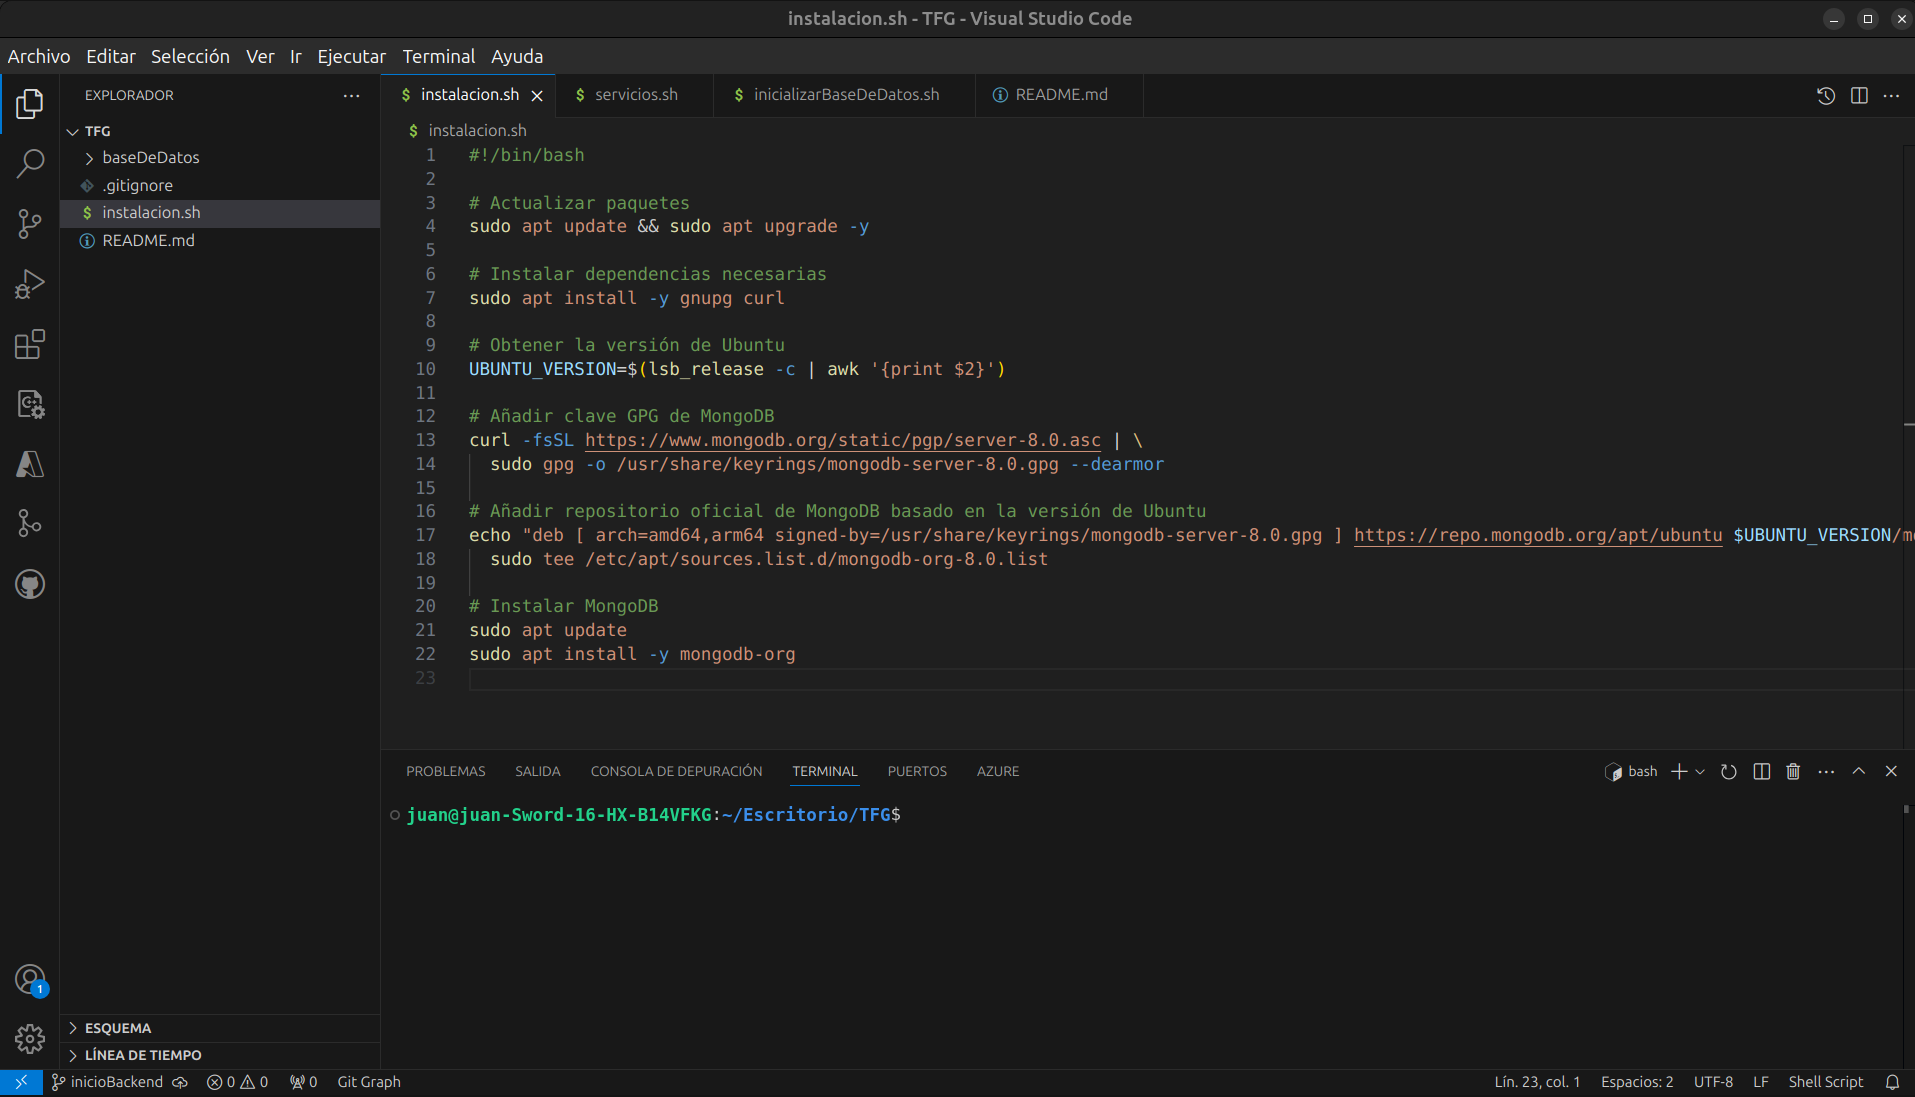
\includegraphics[width=1\linewidth]{imagenes/vc.png}
     \caption[\textbf{Interfaz de Visual Studio Code}.]{\textbf{Interfaz de Visual Studio Code}. Su interfaz es llamativa, limpia, intuitiva y personalizable. Permite ver todos los archivos de manera estructurada, gestionar las ramas de Git y resolver los conflictos de manera fácil y eficiente, entre otras funciones muy útiles.}
     \label{fig:visualStudio-label}
 \end{figure}


\newpage

\section{Base de datos: MongoDB}

Para el almacenamiento de datos en nuestra plataforma, se ha optado por utilizar \textbf{MongoDB}, una base de datos NoSQL ampliamente utilizada debido a su potencia, escalabilidad y flexibilidad. MongoDB almacena los datos en documentos BSON (una representación binaria de JSON), lo cual permite una estructura de datos más dinámica en comparación con las bases de datos relacionales tradicionales.

Una de las principales ventajas de MongoDB es su capacidad para manejar documentos con esquemas variables. Por ejemplo, un usuario puede tener 20 videojuegos marcados como favoritos, otro usuario solo 5, y otro ninguno, sin que ello suponga un problema a nivel de estructura de base de datos. Además, permite añadir o eliminar campos fácilmente durante el desarrollo sin necesidad de redefinir esquemas rígidos, algo que sería considerablemente más complejo en bases de datos SQL.

Para nuestra plataforma se ha creado una única base de datos denominada \textbf{LangGames} —una combinación de \textit{LangChain} y \textit{video games}— y una colección principal llamada \textbf{Usuarios}, donde se almacenan los perfiles y preferencias de los usuarios.

Con el fin de facilitar la configuración del entorno de desarrollo, se han creado tres scripts bash:

\begin{itemize}
	\item Un script para la instalación de MongoDB, que configura los repositorios oficiales y realiza la instalación de los paquetes necesarios.
	\item Un script para lanzar y habilitar el servicio de MongoDB al inicio del sistema.
	\item Un script que inicializa la base de datos \textit{LangGames} y crea la colección \textit{Usuarios}, asegurando que el sistema esté listo para su uso desde el primer momento.
\end{itemize}

\begin{figure}[H]
	\centering
	
\includegraphics[width=1\linewidth]{imagenes/mongoDBLogo.png}
	\caption[\textbf{Logo de MongoDB}.]{\textbf{Logo de MongoDB}. MongoDB es una base de datos orientada a documentos, altamente flexible y escalable, ideal para el desarrollo ágil de aplicaciones. \href{https://www.ovhcloud.com/sites/default/files/styles/large_screens_1x/public/2022-03/black.png}{https://www.ovhcloud.com/sites/default/files/styles/large\_screens\_1x/public/2022-03/black.png}.}
	\label{fig:mongodb-logo}
\end{figure}


\newpage

\section{BackEnd: Python, FastAPI y LangChain}

El backend de la plataforma ha sido desarrollado en \textbf{Python}, un lenguaje de programación interpretado, multiparadigma y de alto nivel. Su sintaxis sencilla y su extensa comunidad lo han posicionado como una de las principales opciones en el desarrollo de software moderno, especialmente en áreas como la inteligencia artificial, ciencia de datos y desarrollo web.

\begin{figure}[H]
	\centering
	
\includegraphics[width=0.5\linewidth]{imagenes/pythonLogo.png}
	\caption[\textbf{Logo de Python}.]{\textbf{Logo de Python}. Python es uno de los lenguajes de programación más populares y versátiles del panorama actual. \href{https://upload.wikimedia.org/wikipedia/commons/thumb/c/c3/Python-logo-notext.svg/640px-Python-logo-notext.svg.png}{https://upload.wikimedia.org/wikipedia/commons/thumb/c/c3/Python-logo-notext.svg/640px-Python-logo-notext.svg.png}.}
	\label{fig:python-logo}
\end{figure}

Para construir la Api que comunica el backend con el frontend, se ha utilizado la biblioteca \textbf{FastAPI}. Esta herramienta permite definir endpoints de manera declarativa y estructurada, facilitando la validación de datos mediante el uso de modelos definidos con \textit{Pydantic}. Además, gracias a su integración con herramientas como OpenAPI, proporciona una documentación automática e interactiva.

El servidor de desarrollo que ejecuta la aplicación FastAPI se gestiona mediante \textbf{Uvicorn}, un servidor ASGI (Asynchronous Server Gateway Interface) ligero y de alto rendimiento, especialmente diseñado para aplicaciones web modernas basadas en Python asíncrono.

\begin{figure}[H]
	\centering
	
\includegraphics[width=1\linewidth]{imagenes/fastapiLogo.png}
	\caption[\textbf{Logo de FastAPI}.]{\textbf{Logo de FastAPI}. FastAPI es una potente biblioteca de Python que permite construir APIs de forma rápida, sencilla y robusta. \href{https://miro.medium.com/v2/resize:fit:1200/1*gTztqjO7u5-GVx2cowVPsA.png}{https://miro.medium.com/v2/resize:fit:1200/1*gTztqjO7u5-GVx2cowVPsA.png}.}
	\label{fig:fastapi-logo}
\end{figure}

Para mantener un entorno limpio y controlado, se utiliza un \textbf{entorno virtual} de Python, el cual permite aislar las dependencias del proyecto del resto del sistema. Esto evita conflictos entre bibliotecas y facilita la portabilidad del entorno de desarrollo.

El backend incluye dos scripts bash:

\begin{itemize}
	\item \textbf{Script de instalación de Python y pip}: actualiza los paquetes del sistema e instala Python 3 junto con \texttt{pip} (el gestor de paquetes de Python) y \texttt{venv} (módulo para entornos virtuales).
	
	\item \textbf{Script de inicialización del entorno}: crea y activa un entorno virtual si no existe, instala todas las dependencias necesarias para el backend (incluyendo FastAPI, Uvicorn, LangChain y otras bibliotecas auxiliares), genera un archivo \texttt{requirements.txt} con la lista de dependencias, y lanza el servidor FastAPI en segundo plano, redirigiendo su salida a un archivo de log.
\end{itemize}

Dentro del backend se encuentra el archivo principal \texttt{main.py}, la carpeta \texttt{app/} que contiene los distintos módulos del sistema, y un archivo de entorno(.env) adicional para gestionar claves necesarias para el correcto funcionamiento de ciertas funcionalidades, cuya obtención y uso está debidamente documentada en el \texttt{README} del repositorio de GitHub.

A continuación, se describe con mayor detalle la estructura y funcionalidad de la carpeta \texttt{app/}.


\subsection{DB}

La carpeta \texttt{db} contiene un único archivo llamado \texttt{mongodb.py}, el cual se encarga de gestionar la conexión con la base de datos MongoDB.

En él se utiliza la biblioteca \texttt{pymongo} para establecer la conexión con el servidor local de MongoDB (\texttt{localhost:27017}). Una vez conectados, se selecciona la base de datos \texttt{LangGames} y se almacena la colección \texttt{Usuarios} en una variable que se puede importar fácilmente desde otros módulos del backend.

Esta estrategia favorece la reutilización y centralización del acceso a la base de datos, evitando duplicación de código y facilitando su mantenimiento.


\subsection{Utils}

Esta carpeta contiene dos archivos con funciones auxiliares esenciales para el funcionamiento del backend.

\begin{itemize}
	\item \textbf{jwt.py}: Este archivo se encarga de generar \textbf{tokens JWT (JSON Web Tokens)}, que permiten autenticar de forma segura a los usuarios. Cada vez que un usuario inicia sesión correctamente, se le genera un token que contiene su correo electrónico (u otro dato identificativo) y una fecha de expiración. Este token se firma digitalmente usando una clave secreta, de modo que el servidor pueda verificar su validez en futuras peticiones sin necesidad de mantener sesiones abiertas. Así se garantiza una comunicación segura y sin estado entre el cliente y el servidor.
	
	\item \textbf{utilidadesVarias.py}: Aquí se agrupan funciones y configuraciones de utilidad. Por ejemplo:
	\begin{itemize}
		\item Se cargan las claves necesarias para acceder a las APIs externas desde un archivo \texttt{.env}.
		\item Se definen listas con los modelos de lenguaje disponibles para su uso.
		\item \texttt{limpiar\_respuesta()}: una función que extrae y limpia la parte JSON de las respuestas generadas por modelos de lenguaje.
		\item \texttt{obtener\_imagen\_juego()}: consulta la API de RAWG para obtener automáticamente una imagen representativa del videojuego que se le indique.
	\end{itemize}
\end{itemize}


\subsection{Modelos}

Los modelos representan la estructura de los datos con los que trabaja el sistema, facilitando la organización y el intercambio de información entre distintas partes del backend.

El modelo principal es el del \textbf{usuario}, que incluye tanto los datos básicos como el nombre, correo y contraseña, como otros campos más específicos relacionados con el mundo de los videojuegos. Por ejemplo, se almacena información sobre las consolas que posee, la configuración de su ordenador, sus gustos personales, los juegos que ha jugado o que no le han gustado, e incluso su historial de los videojuegos recomendados por los modelos de lenguaje. Esta estructura permite personalizar al máximo la experiencia del usuario.

Además del modelo de usuario, se han definido otras clases auxiliares para manejar información concreta:
\begin{itemize}
	\item Modelos para solicitudes de recomendación, tanto básica como personalizada.
	\item Un modelo para representar los próximos lanzamientos de videojuegos, incluyendo su título, fecha, plataformas y una imagen asociada.
\end{itemize}

Estas clases permiten que los distintos módulos del backend se comuniquen utilizando estructuras coherentes y bien definidas, lo que facilita la validación de datos y mejora la organización del código.



\subsection{Gestores}

Los gestores se encargan de realizar las operaciones relacionadas con los datos que maneja el sistema. En este caso, contamos con un gestor centrado en los usuarios.

El \textbf{gestor de usuarios} proporciona una serie de funciones que permiten crear un nuevo usuario, obtener sus datos, modificarlos o eliminarlos. También incluye la verificación de contraseñas para el proceso de inicio de sesión y una función para limpiar los campos opcionales del perfil del usuario. Además aplica un hash a las contraseñas para que el sistema sea más seguro.

Este archivo actúa como intermediario entre la base de datos y otras partes de la aplicación, como las rutas o los servicios. Gracias a él, se centraliza la lógica relacionada con los usuarios, facilitando el mantenimiento y la reutilización del código.


\subsection{Servicios}

Los servicios se encargan de implementar las funcionalidades centrales del sistema.

El servicio de usuario actúa como intermediario entre el gestor de usuarios y los demás servicios. Su función principal es preprocesar los datos recibidos del usuario, invocar los servicios correspondientes con dichos datos y aplicar las modificaciones necesarias en el perfil.

El servicio de recomendación básica está diseñado para usuarios no autenticados que solicitan recomendaciones de videojuegos. Ante una petición, se consultan hasta tres modelos de lenguaje para obtener posibles respuestas. Si algún modelo falla, el sistema puede seguir con normalidad. Una vez obtenidas las respuestas, un modelo la sintetiza en una sola. Si el modelo falla, se sigue con los siguientes hasta que se obtiene una respuesta válida. Esta gestión secuencial de modelos se facilita mediante la biblioteca \texttt{LangChain}, que simplifica la invocación, manejo y conmutación entre modelos. Para acceder a los modelos, se utiliza \texttt{OpenRouter}, una API que permite interactuar con múltiples proveedores y modelos sin necesidad de gestionar varias claves de acceso. \texttt{OpenRouter} también ofrece una prueba gratuita limitada en tokens.

El servicio de recomendación personalizada extiende la funcionalidad básica incorporando datos específicos del usuario, como su historial de videojuegos y recomendaciones previas, para evitar redundancias. Además, este servicio puede actualizar el perfil del usuario automáticamente si la petición incluye información que modifica su estado, como la venta de una consola o la adquisición de un nuevo juego.

Por otro lado, existe un servicio dedicado exclusivamente a actualizar la información relativa a los videojuegos del usuario a partir del texto que éste proporciona. Este servicio utiliza modelos de lenguaje para analizar la petición y detectar los cambios necesarios, devolviendo una actualización precisa y estructurada.

Asimismo, contamos con dos servicios innovadores que mejoran significativamente la experiencia de usuario:

\begin{enumerate}
	\item \textbf{Servicio de próximos lanzamientos:} Este servicio obtiene información sobre videojuegos próximos a salir mediante la API de RAWG, incluyendo nombres, géneros, plataformas y imágenes. Los modelos analizan estos datos para filtrar y recomendar aquellos títulos que mejor se ajustan a los gustos del usuario.
	\item \textbf{Servicio de integración con Steam:} Mediante la API de Steam, este servicio recupera la lista de juegos poseídos por el usuario y el tiempo de juego asociado a cada uno, usando su ID de Steam. Basándonos en esta información, actualizamos el perfil del usuario, considerando que un juego está realmente jugado si el usuario ha dedicado más de una hora a jugarlo.
\end{enumerate}

\subsection{Rutas}

Las rutas permiten exponer las funcionalidades del sistema a través de peticiones HTTP, especificando el tipo de operación (\texttt{GET}, \texttt{POST}, \texttt{PUT}, \texttt{DELETE}), la ruta asociada (path), los posibles errores, y los datos requeridos o devueltos. Estas rutas actúan como puntos de entrada a los servicios internos de la aplicación, es decir, el controlador.

En el sistema se han definido rutas para distintas funcionalidades clave:

\begin{itemize}
	\item \textbf{Autenticación:} Permite a los usuarios iniciar sesión mediante la verificación de credenciales. Al autenticarse correctamente, se genera y devuelve un token JWT que puede ser utilizado en peticiones protegidas.
	
	\item \textbf{Gestión de usuarios:} Incluye rutas para crear, obtener, actualizar y eliminar usuarios, así como para modificar sus datos obligatorios u opcionales, acceder a sus preferencias y sincronizar sus datos con Steam.
	
	\item \textbf{Recomendaciones:} Ofrece rutas tanto para recomendaciones básicas (sin necesidad de estar autenticado) como para recomendaciones personalizadas basadas en el perfil y el historial del usuario.
	
	\item \textbf{Próximos lanzamientos:} Permite obtener una lista de videojuegos próximos a lanzarse, filtrados en función de los gustos del usuario, utilizando datos de la API de RAWG.
\end{itemize}

Cada ruta está asociada a un módulo independiente dentro de la aplicación, lo que favorece una organización modular y facilita el mantenimiento y la ampliación del sistema.

\subsection{Main}

El archivo \texttt{main.py} actúa como punto de entrada de la aplicación. Su función principal es inicializar el servidor web y registrar todas las rutas disponibles en el sistema. Para ello, importa los distintos módulos de rutas definidos en la aplicación y los incluye en la instancia principal de \texttt{FastAPI} mediante el método \texttt{include\_router()}.

Además, se configura el middleware de CORS (\textit{Cross-Origin Resource Sharing}) para permitir que la aplicación frontend (por ejemplo, una interfaz en Angular corriendo en \texttt{http://localhost:4200}) pueda comunicarse con el backend sin restricciones de origen.

Este archivo es esencial para arrancar el sistema y exponer todos los servicios a través de una única instancia centralizada.


\newpage

\section{FrontEnd: Angular}

El frontend de la aplicación ha sido desarrollado utilizando \textbf{Angular}, un framework de desarrollo web moderno, mantenido por Google, que facilita la creación de aplicaciones de una sola página (SPA) con una arquitectura robusta y escalable.

Angular se basa principalmente en los lenguajes \textbf{HTML}, \textbf{SCSS/CSS} y \textbf{TypeScript}. Para el diseño visual y la personalización del estilo, se ha utilizado el framework de utilidades CSS \textbf{Tailwind CSS}, que permite construir interfaces de usuario de forma rápida y flexible mediante clases predefinidas.

Al igual que las otras partes cuenta con scripts, para instalar lo necesario e inicializar el frontend en segundo plano. También cuenta con un script que se utilizó para comenzar el desarrollo.

Estos scripts simplifican considerablemente el proceso de despliegue local, garantizando que cualquier desarrollador pueda ejecutar el frontend con facilidad.

\begin{figure}[H]
	\centering
	
\includegraphics[width=1\linewidth]{imagenes/logoAngular.png}
	\caption[\textbf{Logo de Angular}.]{\textbf{Logo de Angular}. Angular es un framework completo y muy utilizado para el desarrollo de interfaces web modernas. Fuente: \href{https://media.licdn.com/dms/image/v2/D4D12AQHF0nuL7dxEOA/article-cover_image-shrink_720_1280/article-cover_image-shrink_720_1280/0/1710076882649?e=2147483647&v=beta&t=z_GWbz1UXR5oIm-mSUhdCJnspOV0vronhDj9-o7xOhI}{https://media.licdn.com/dms/image/v2/D4D12AQHF0nuL7dxEOA/article-cover\_image-shrink\_720\_1280/article-cover\_image-shrink\_720\_1280/0/1710076882649?e=2147483647\&v=beta\&t=z\_GWbz1UXR5oIm-mSUhdCJnspOV0vronhDj9-o7xOhI}.}
	\label{fig:logo-angular}
\end{figure}


Angular genera automáticamente gran parte de la estructura inicial del proyecto, lo cual permite centrarse desde el inicio en el desarrollo funcional y visual de la aplicación.

Uno de los elementos clave en la personalización del diseño es la configuración del sistema de estilos. Para ello se ha utilizado \textbf{Tailwind CSS}, que ofrece una forma muy eficiente y flexible de aplicar estilos directamente en los componentes. En este caso, se ha habilitado el modo claro y oscuro, de forma que el diseño se adapta según las preferencias del usuario. Además, se han realizado pequeños ajustes para asegurar que, incluso en campos de formularios autocompletados, los colores se mantengan coherentes con el tema activo.

La estructura principal del frontend se encuentra en la carpeta src donde reside el código fuente. Allí se definen aspectos globales como el título de la página, el icono del navegador, la dirección base de la API y los estilos que afectan a toda la aplicación.

Dentro de esta estructura se encuentra la carpeta principal del proyecto, app, que es donde se desarrolla casi toda la funcionalidad. Esta parte incluye, por ejemplo, la definición de las rutas de navegación, que permiten moverse entre las distintas vistas como el inicio, el registro o la pantalla principal tras iniciar sesión.

También se incluye un sistema de servicios en la carpeta services, que se encargan de gestionar las conexiones con la API. Uno de estos servicios, por ejemplo, permite obtener los próximos lanzamientos de videojuegos relacionados con el usuario. Estos datos se almacenan temporalmente en memoria caché para evitar repetir llamadas innecesarias, lo que mejora la eficiencia y la velocidad de la aplicación.

Además, se han definido varias \textbf{interfaces} que actúan como plantillas para los datos que se van a utilizar, como pueden ser las recomendaciones personalizadas, los lanzamientos futuros o los datos de los usuarios. Estas interfaces permiten trabajar con los datos de forma más organizada y segura.

A continuación, se describe la carpeta de \textit{componentes}, que contiene las diferentes piezas visuales y funcionales que forman la interfaz del sistema.

\subsection{Componentes}

En Angular, un componente es una de las piezas clave para construir interfaces. Cada uno representa una parte específica de la aplicación y cuenta con su propia estructura (HTML), comportamiento (TypeScript) y estilo (CSS o SCSS). Gracias a la modularidad que ofrece este enfoque, podemos construir interfaces complejas a partir de componentes más simples y reutilizables.

En nuestro caso, todos los componentes han sido diseñados pensando en la experiencia del usuario. Incluyen un botón para alternar entre modo claro y oscuro, se adaptan automáticamente a pantallas pequeñas (diseño responsive), e incorporan pequeñas animaciones que hacen la experiencia más agradable. Por ejemplo, se utiliza una Poké Ball giratoria durante las cargas normales, y un R2D2 para mostrar mientras carga los próximos lanzamientos.

A continuación, describimos cada componente de forma individual.

\subsubsection{Home}

El componente \texttt{Home} es la página principal de la aplicación. Nada más entrar, el usuario se encuentra con una cabecera que incluye el nombre de la app, su logotipo, y dos botones: uno para iniciar sesión y otro para registrarse.

En el centro de la página hay un cuadro de texto donde el usuario puede escribir qué tipo de juego está buscando. Una vez enviada la petición, se muestran las recomendaciones en formato de tarjetas. Cada tarjeta incluye una imagen del juego, su nombre, las plataformas disponibles y una breve explicación de por qué se ha recomendado ese juego en concreto.

En la parte inferior, se encuentra una sección con un segundo logotipo y el aviso de derechos de autor.

\vspace{0.5cm}

\begin{figure}[H]
	\centering
	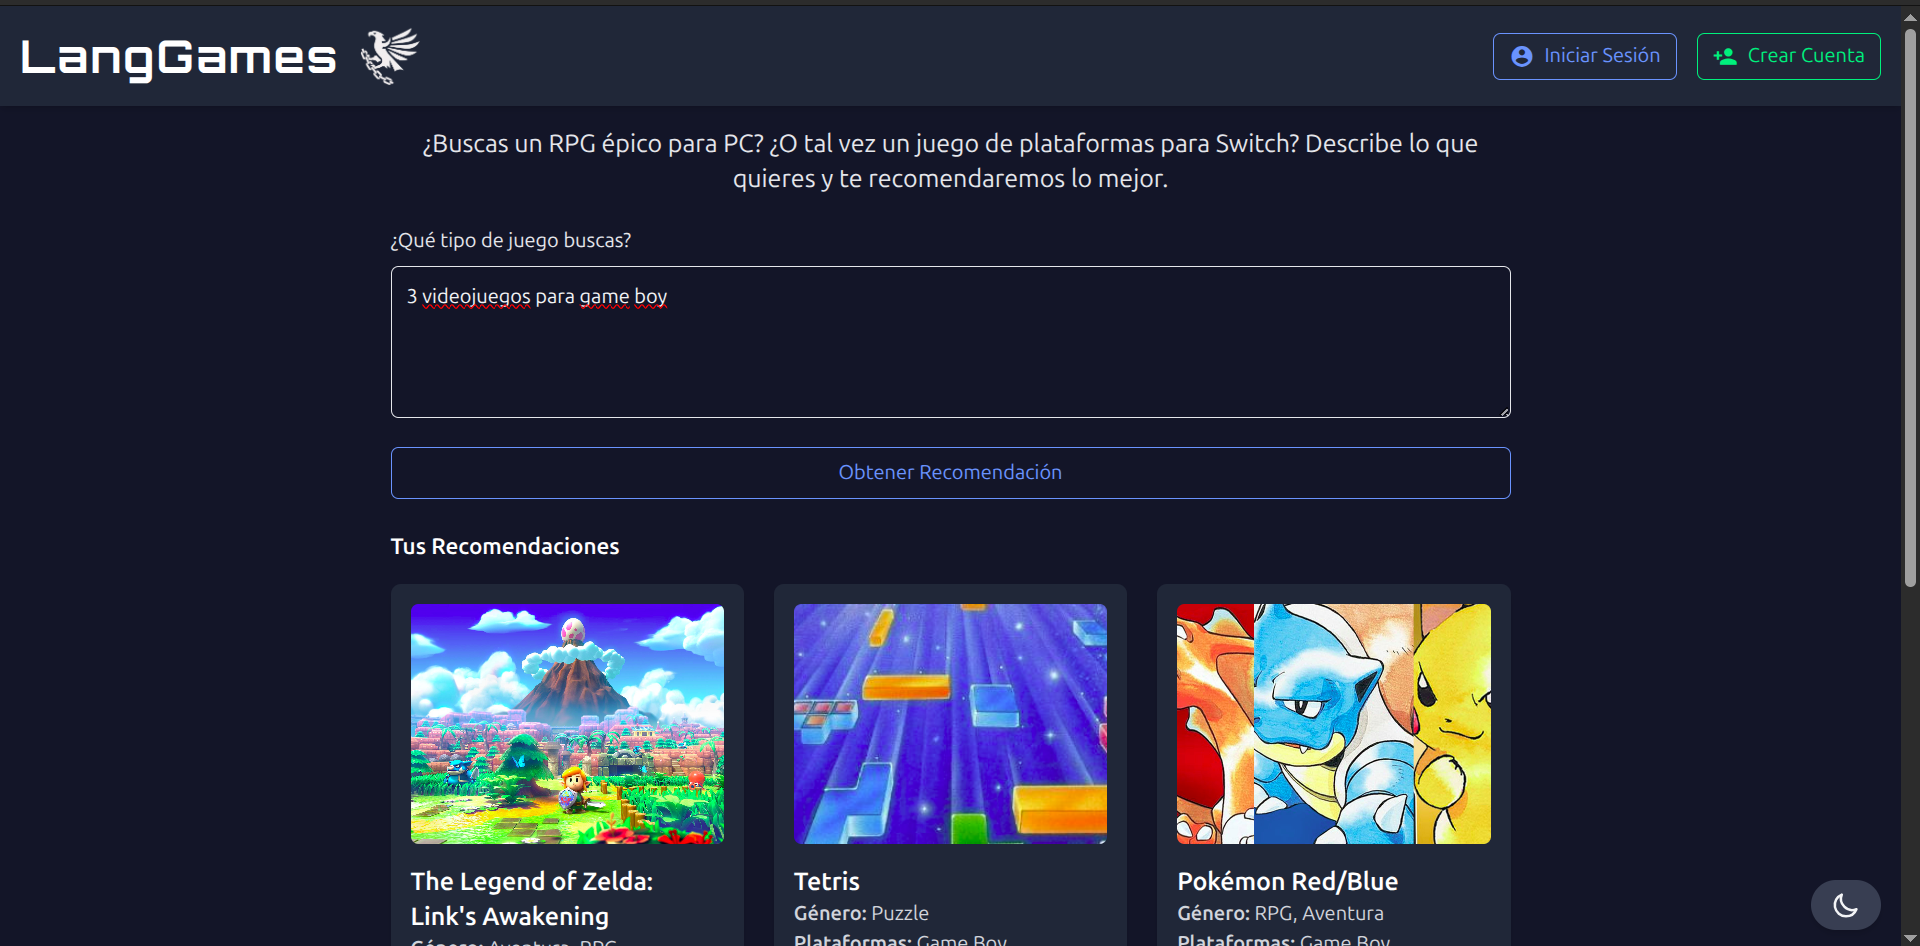
\includegraphics[width=1\linewidth]{imagenes/home1.png}
	\caption[\textbf{Imagen de home 1}.]{\textbf{Imagen de home 1}. Vista principal de la página con recomendaciones ya generadas.}
	\label{imagen-home-1}
\end{figure}

\begin{figure}[H]
	\centering
	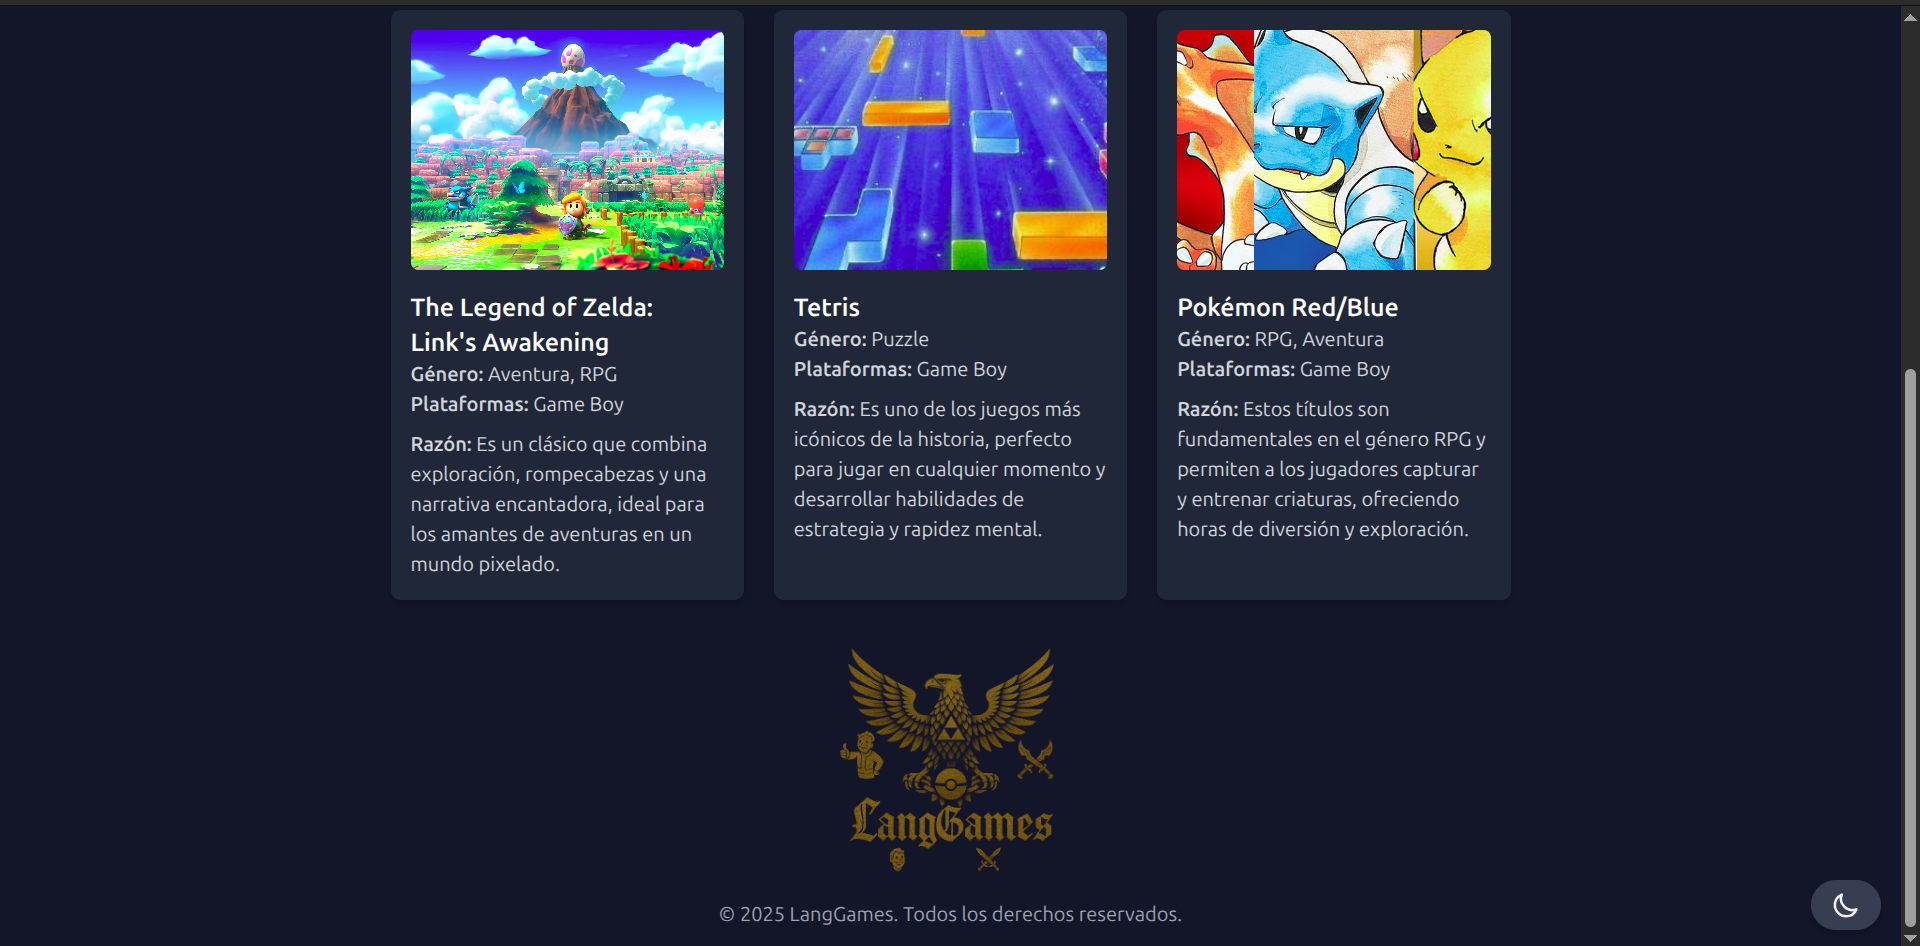
\includegraphics[width=1\linewidth]{imagenes/home2.png}
	\caption[\textbf{Imagen de home 2}.]{\textbf{Imagen de home 2}. Parte inferior de la página, con el segundo logotipo y el pie de página.}
	\label{imagen-home-2}
\end{figure}

\begin{figure}[H]
	\centering
	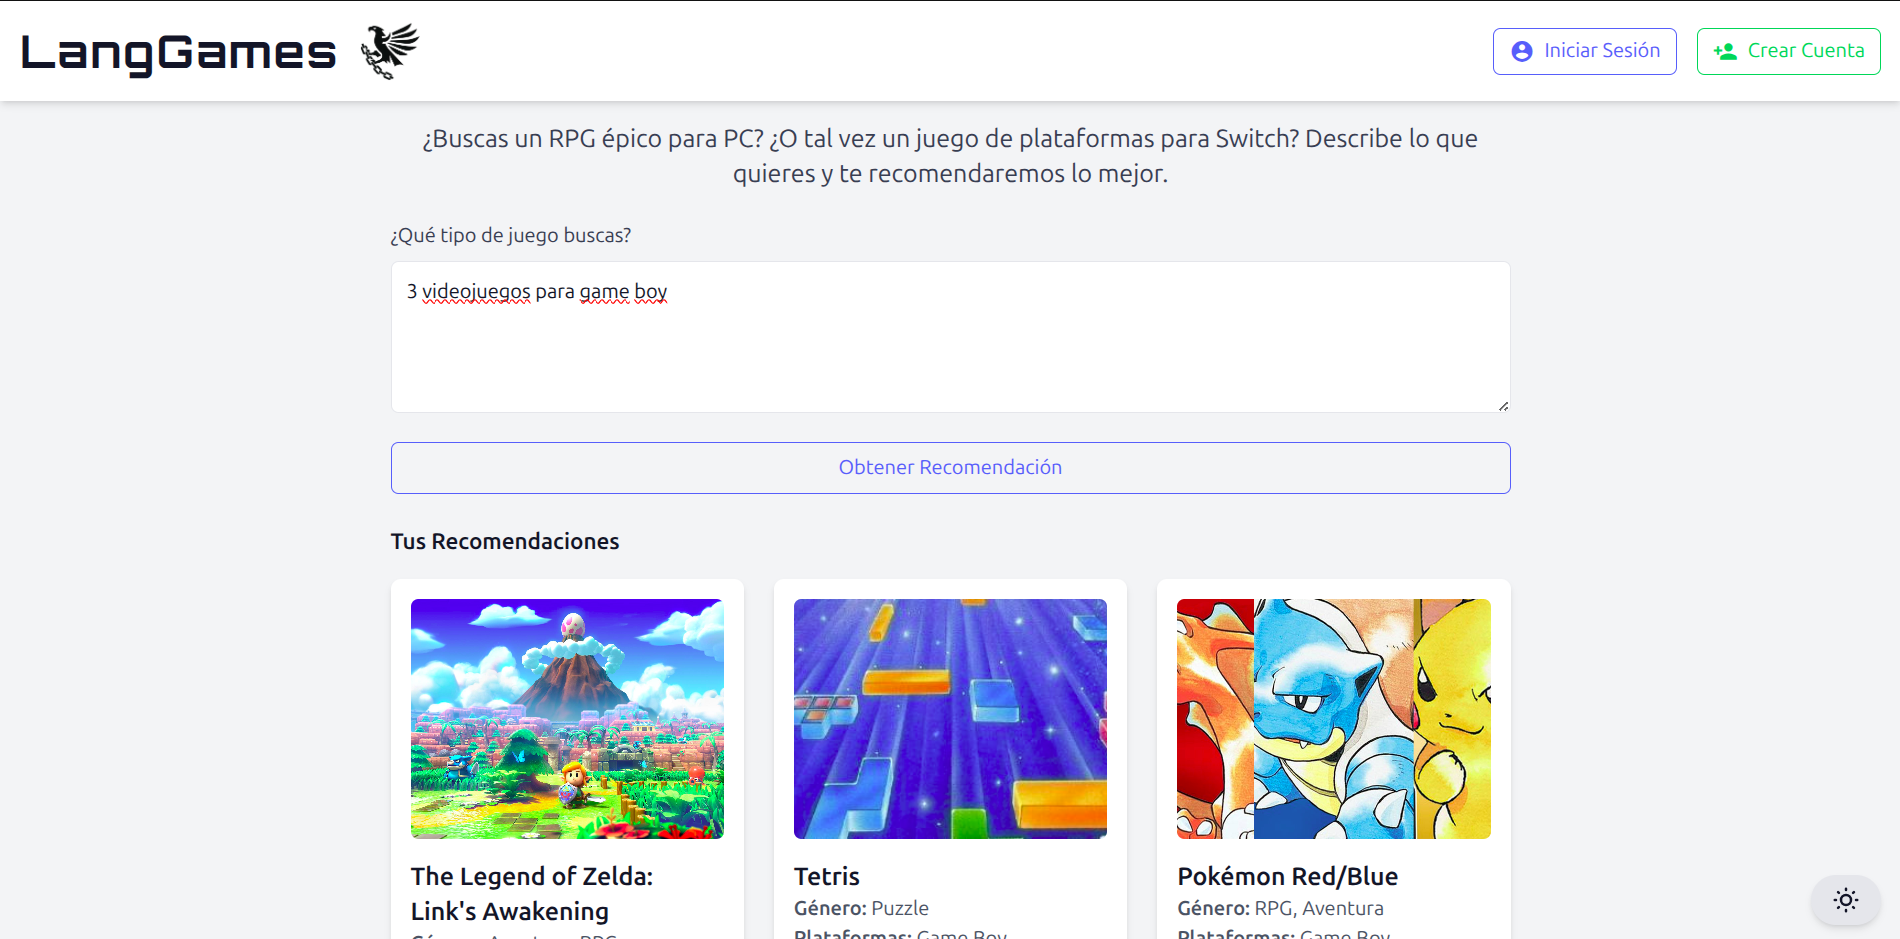
\includegraphics[width=1\linewidth]{imagenes/homeClaro.png}
	\caption[\textbf{Modo claro}.]{\textbf{Modo claro}. La aplicación ofrece tanto modo claro como oscuro, para mayor comodidad del usuario.}
	\label{imagen-home-claro}
\end{figure}

\begin{figure}[H]
	\centering
	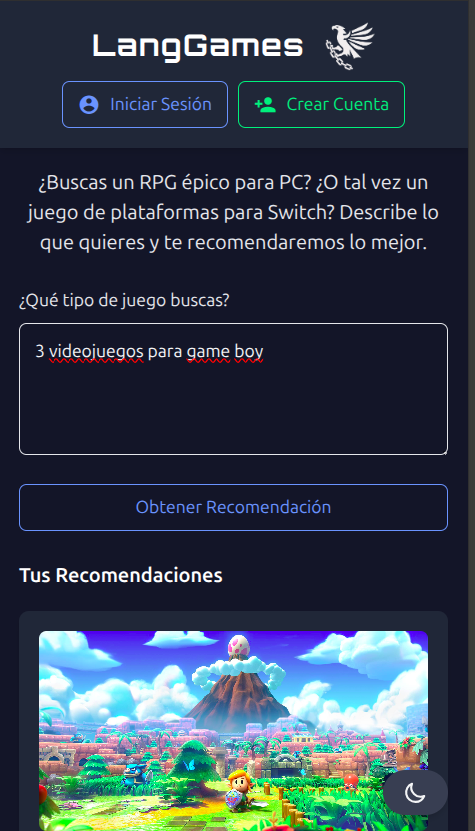
\includegraphics[width=1\linewidth]{imagenes/homeMovil1.png}
	\caption[\textbf{Vista móvil 1}.]{\textbf{Vista móvil 1}. Diseño adaptado para dispositivos móviles, con todos los elementos reorganizados.}
	\label{imagen-movil-1}
\end{figure}

\begin{figure}[H]
	\centering
	
\includegraphics[width=1\linewidth]{imagenes/homeMovil2.png}
	\caption[\textbf{Vista móvil 2}.]{\textbf{Vista móvil 2}. Otra vista desde un dispositivo móvil, mostrando el aspecto del pie de página.}
	\label{imagen-movil-2}
\end{figure}



\subsubsection{Registro}

El sistema de registro permite a los usuarios crear una cuenta nueva desde una ventana superpuesta a la pantalla principal \textit{Home}. Para completar el registro, el usuario debe proporcionar un nombre de usuario, una dirección de correo electrónico válida y una contraseña segura.

El formulario valida en tiempo real que tanto el nombre como el correo electrónico no estén ya registrados en el sistema. En caso contrario, se muestra un mensaje de error al usuario indicando el conflicto.

En cuanto a la contraseña, esta debe cumplir con los siguientes requisitos mínimos:
\begin{itemize}
	\item Tener una longitud mínima de 8 caracteres.
	\item Incluir al menos una letra y un número.
\end{itemize}

Una vez completado el formulario de manera correcta y superadas todas las validaciones, el sistema crea la cuenta de usuario y realiza el inicio de sesión de forma automática, redirigiendo al usuario a la pantalla principal.

\begin{figure}[H]
	\centering
	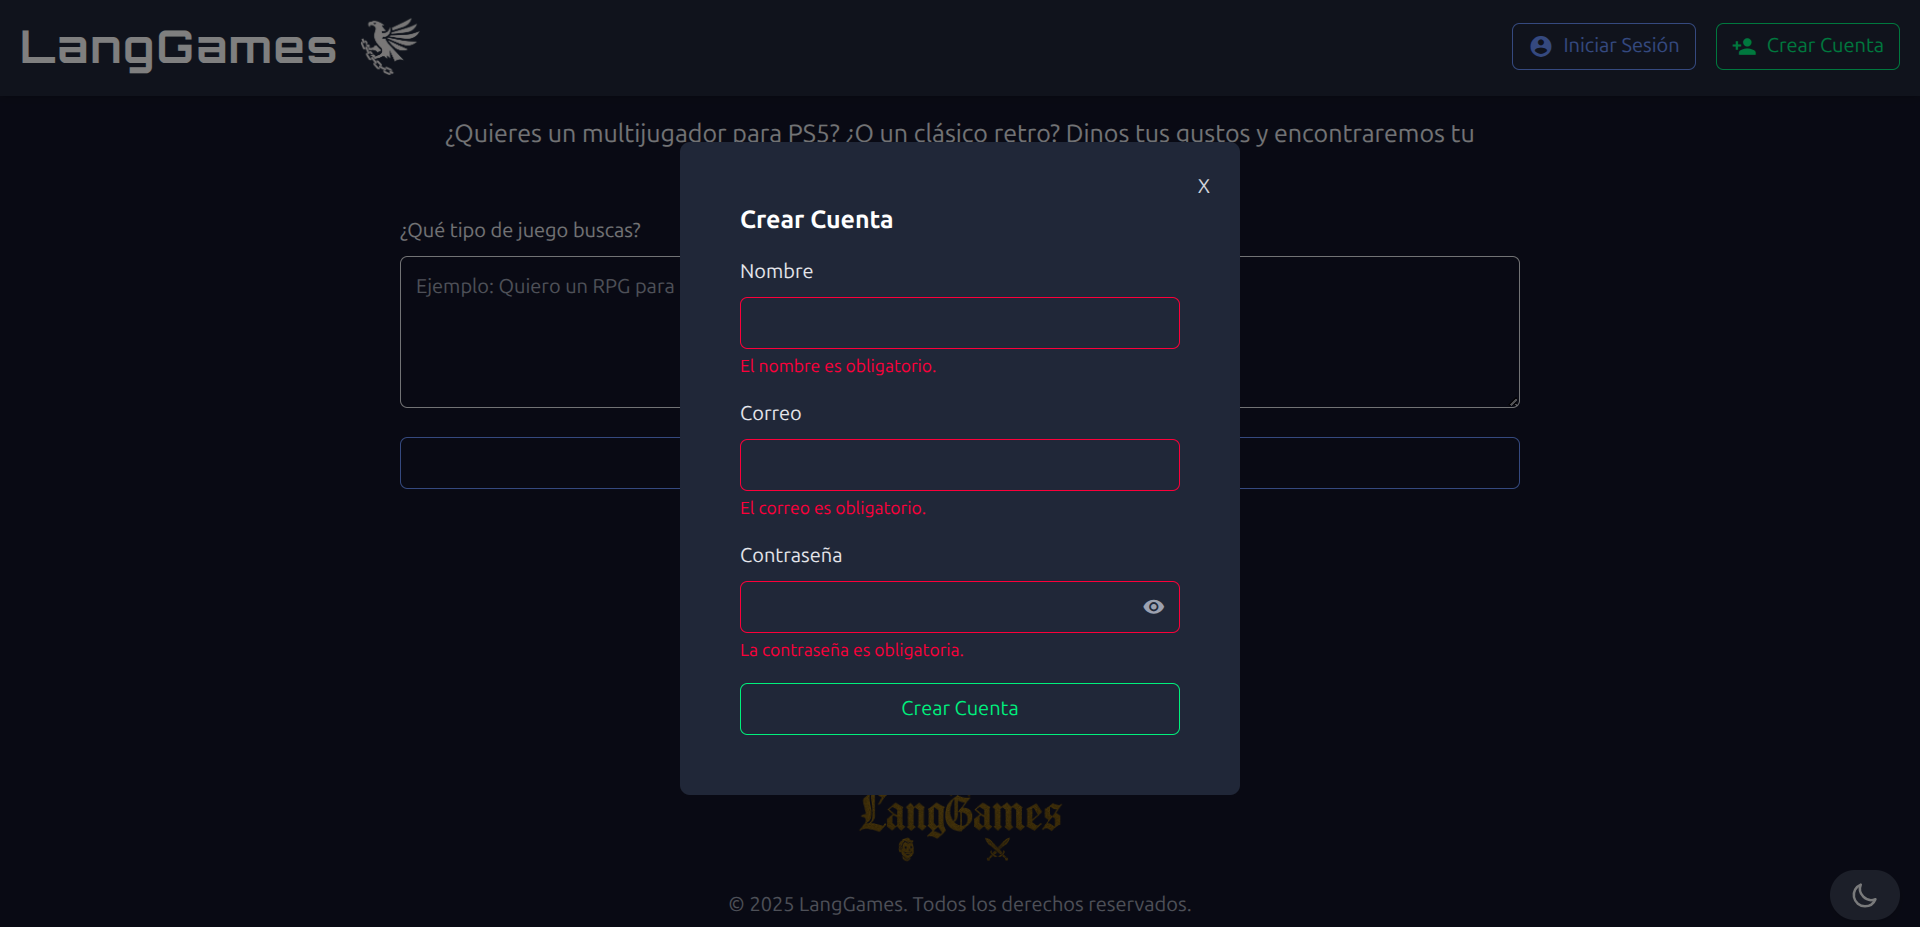
\includegraphics[width=1\linewidth]{imagenes/register.png}
	\caption[\textbf{Registro}.]{\textbf{Registro}. Formulario de creación de cuenta en la plataforma.}
	\label{imagen-register}
\end{figure}



\subsubsection{Login}

El componente de \textit{login} permite a los usuarios autenticarse en la plataforma introduciendo sus credenciales: correo electrónico y contraseña. El formulario verifica que los campos no estén vacíos y que el correo tenga un formato válido antes de enviar los datos.

En caso de que el usuario introduzca credenciales incorrectas o no esté registrado, se muestra un mensaje de error informativo. Si la autenticación es exitosa, se almacena el token de sesión, el rol del usuario, su nombre y su correo en el almacenamiento local del navegador, y se redirige automáticamente a la pantalla principal.

Además, el campo de contraseña ofrece la opción de mostrar u ocultar el texto introducido para mejorar la experiencia del usuario.

\begin{figure}[H]
	\centering
	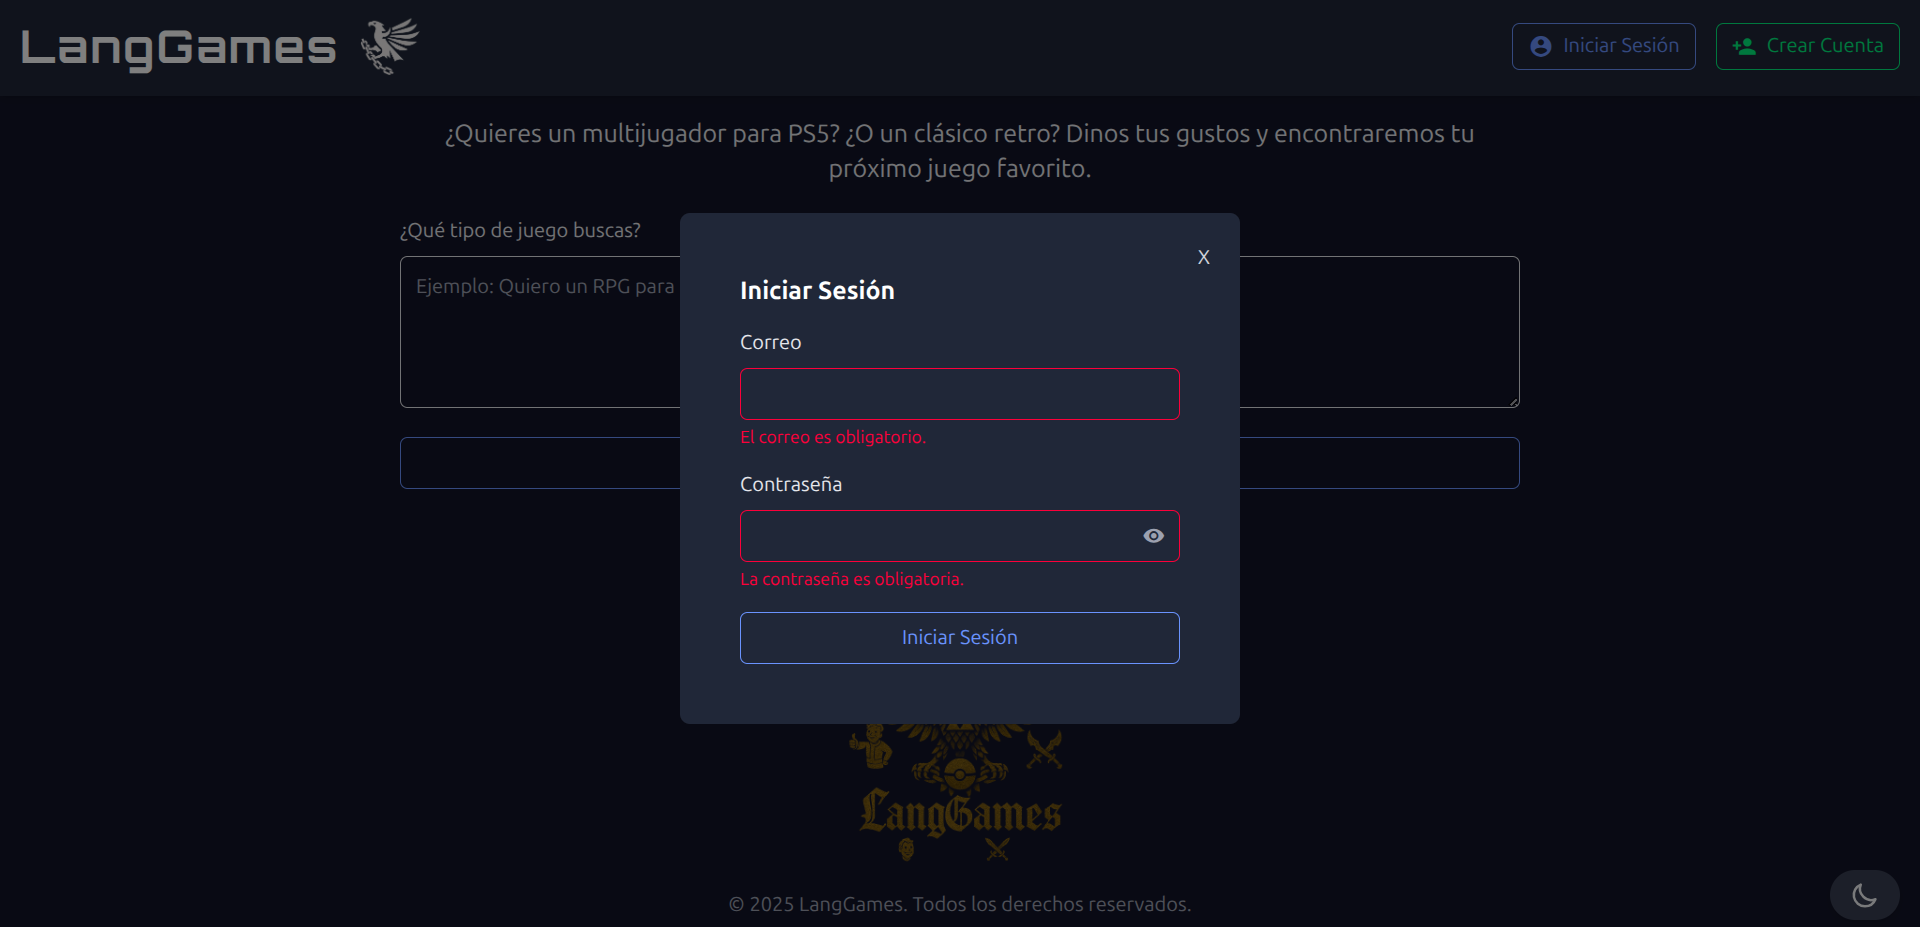
\includegraphics[width=1\linewidth]{imagenes/login.png}
	\caption[\textbf{Inicio de sesión}.]{\textbf{Inicio de sesión}. Formulario para iniciar sesión en la plataforma.}
	\label{imagen-login}
\end{figure}



\subsubsection{Principal}

Este es el componente principal de la aplicación, al que accede el usuario tras iniciar sesión o crear una cuenta.

La interfaz principal incluye una barra superior que muestra el nombre y el logotipo de la plataforma, así como un mensaje de bienvenida personalizado con el nombre del usuario. Además, se incorporan dos botones: uno para acceder a los ajustes de la cuenta y otro para cerrar sesión.

En la parte izquierda de la pantalla se muestran los cuatro próximos lanzamientos. Justo debajo, se encuentran las seis últimas recomendaciones disponibles. En el lateral derecho, hay un cuadro de texto donde el usuario puede solicitar recomendaciones, las cuales se mostrarán en la parte inferior tras ser generadas.

\begin{figure}[H]
	\centering
	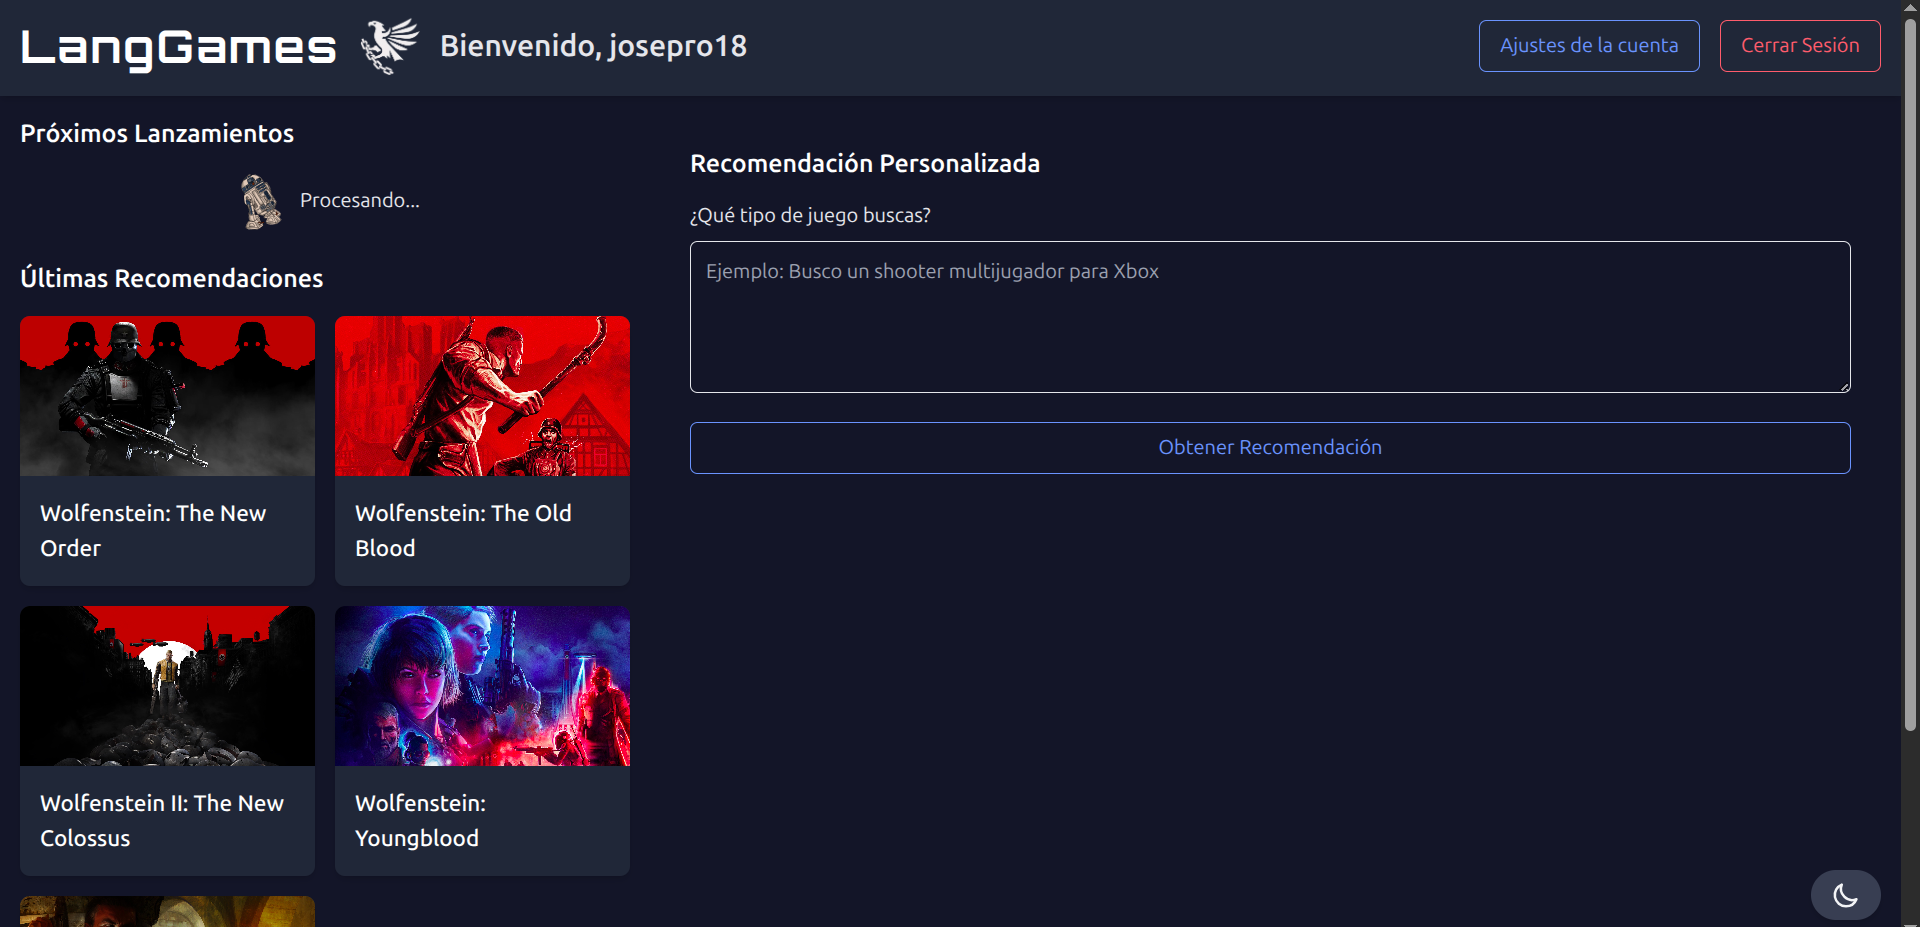
\includegraphics[width=1\linewidth]{imagenes/principal1.png}
	\caption[\textbf{Página principal 1}.]{\textbf{Página principal 1}. Página principal de la plataforma.}
	\label{imagen-principal-1}
\end{figure}

\begin{figure}[H]
	\centering
	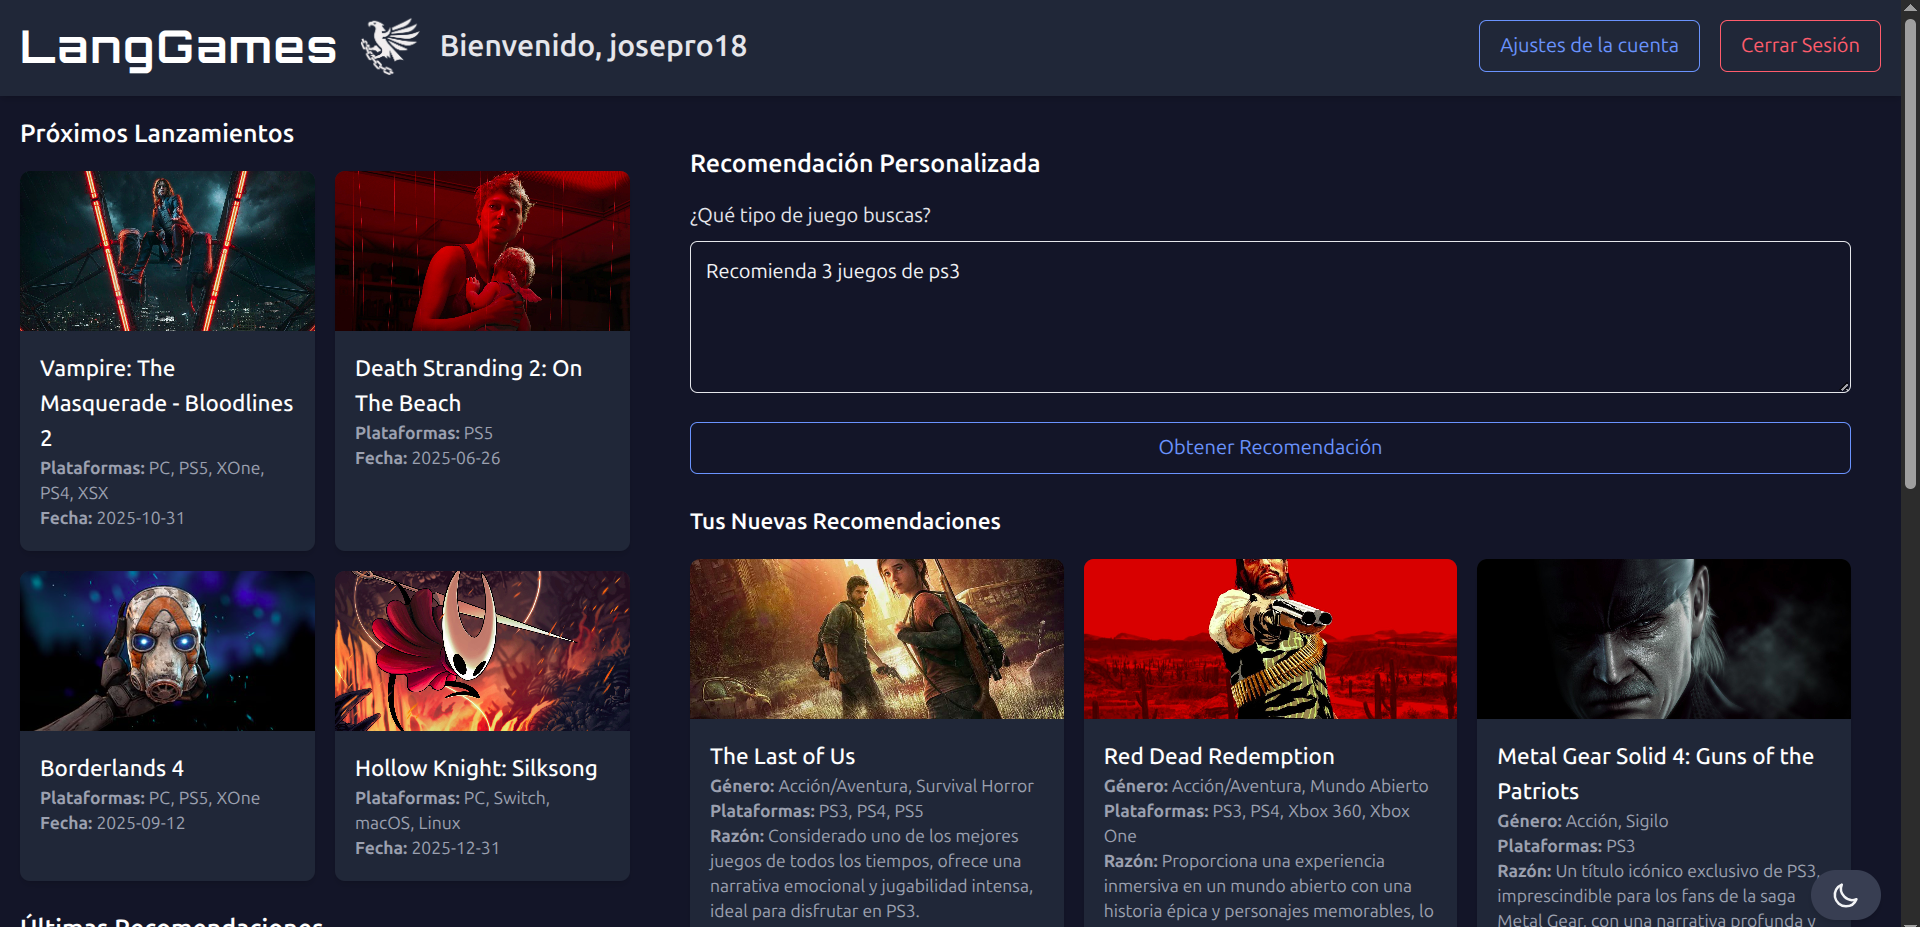
\includegraphics[width=1\linewidth]{imagenes/principal2.png}
	\caption[\textbf{Página principal 2}.]{\textbf{Página principal 2}. Página principal de la plataforma con recomendaciones.}
	\label{imagen-principal-2}
\end{figure}



\subsubsection{Ajustes de cuenta}

La página de ajustes permite al usuario modificar su información personal y gestionar aspectos clave de su cuenta.

En la barra superior se encuentran dos botones: uno para vincular la cuenta con Steam mediante el ID de usuario, y otro para regresar a la página principal.

En la parte izquierda de la página hay otros dos botones. El primero permite cambiar el nombre de usuario y/o la contraseña, o eliminar la cuenta. Para cualquiera de estas acciones, es necesario introducir la contraseña actual. El segundo botón permite restablecer todos los datos relacionados con videojuegos almacenados en la cuenta del usuario. Debajo de estos botones se muestra un resumen con la información sobre los videojuegos del usuario.

En la parte derecha se encuentra un cuadro de texto donde el usuario puede introducir modificaciones mediante lenguaje natural, como por ejemplo indicar la adquisición de una nueva consola o la venta de un juego. El modelo de lenguaje interpreta la petición y aplica la modificación correspondiente, mostrando al usuario un mensaje con el resultado de la operación.

\begin{figure}[H]
	\centering
	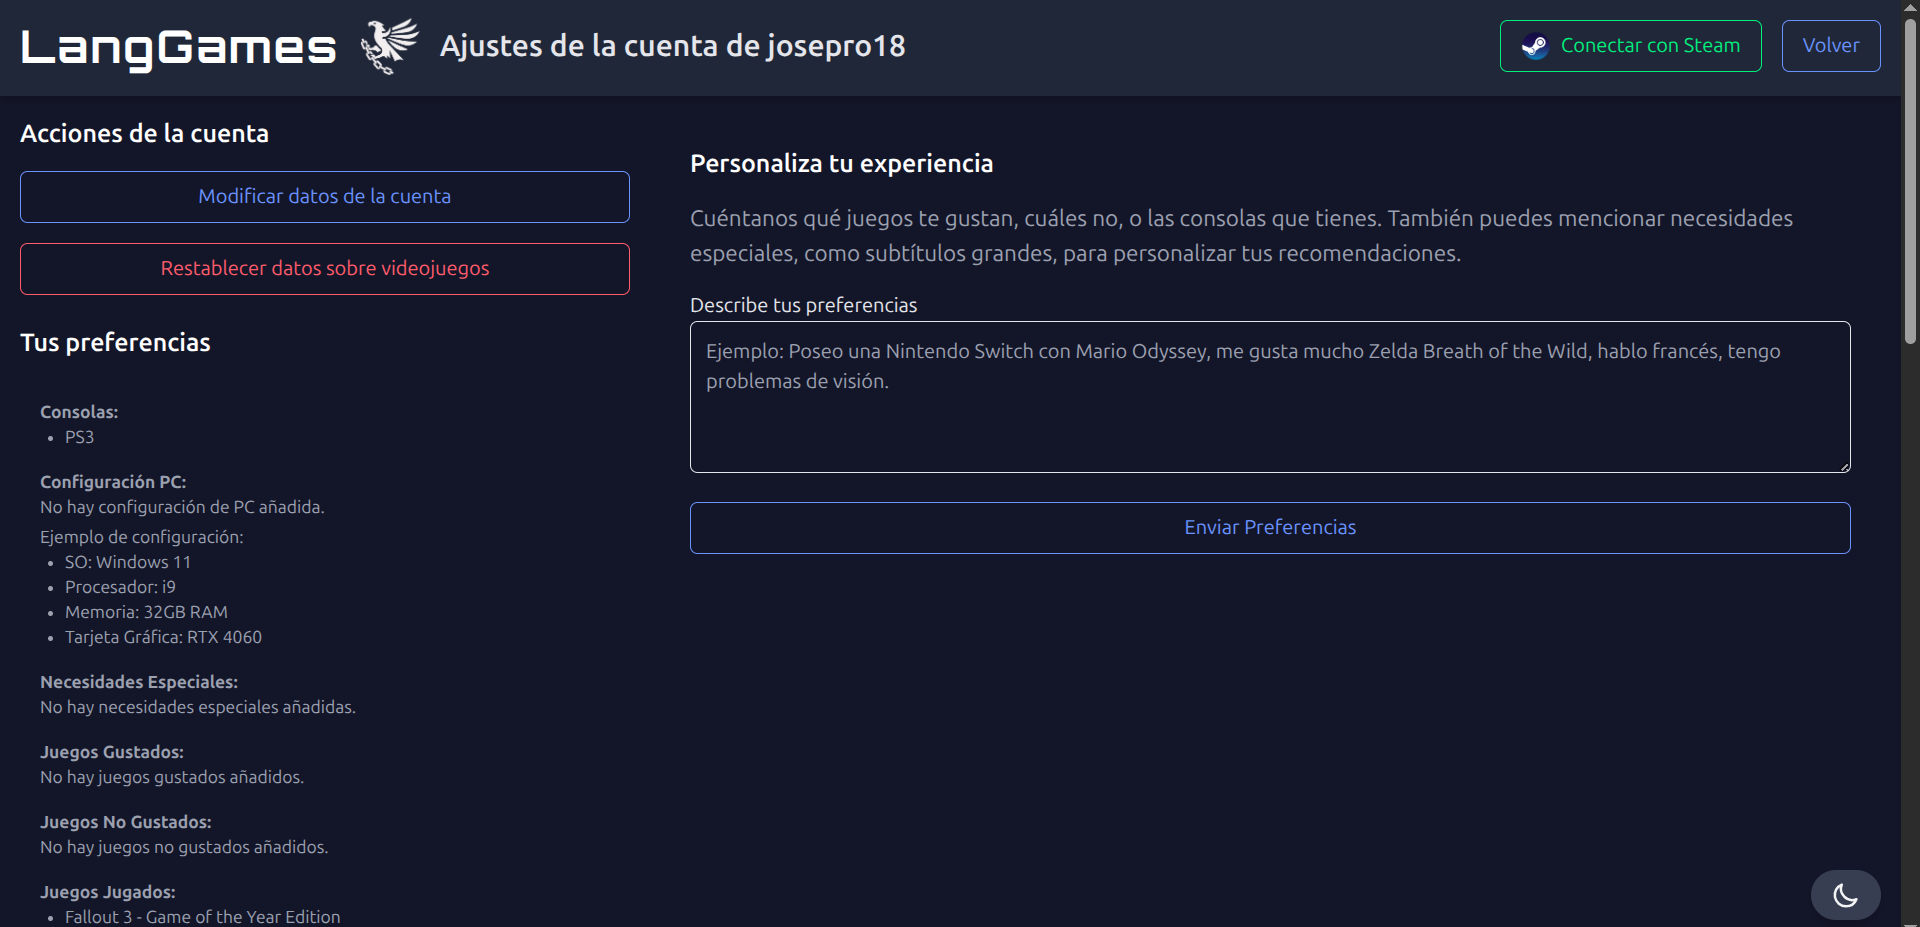
\includegraphics[width=1\linewidth]{imagenes/ajustesCuenta.png}
	\caption[\textbf{Página de ajustes de la cuenta}.]{\textbf{Página de ajustes de la cuenta}. Interfaz donde el usuario puede gestionar la información de su cuenta y realizar ajustes relacionados con sus videojuegos.}
	\label{imagen-ajustes}
\end{figure}

\newpage

\section{Puesta en marcha}

Además, la aplicación incluye tres scripts globales: uno para ejecutar los tres scripts de instalación de los distintos componentes de la plataforma; otro para iniciar el backend y el frontend en segundo plano, almacenando la salida en un archivo de log y guardando sus PIDs para poder detenerlos posteriormente; y un tercer script que permite detener tanto el backend como el frontend que se ejecutan en segundo plano.
